\documentclass[a4paper, 11pt]{article}
\usepackage{lipsum} %This package just generates Lorem Ipsum filler text. 
\usepackage{fullpage} % changes the margin
\usepackage{mathpazo}
\usepackage{multicol}
\usepackage{graphicx}
\usepackage{enumerate}
\usepackage{amsmath,amsfonts,amsthm} % Math packages
\usepackage{listings}
\begin{document}
%Header-Make sure you update this information!!!!
\noindent
\large\textbf{Homework 3} \hfill \textbf{Hongyu Yan (516030910595)} \\
\normalsize {\bf CS 259 Numerical Methods for Data Science} \hfill ACM Class, Zhiyuan College, SJTU\\
Prof.~{\bf David Bindel} \hfill Due Date: June 22nd, 2018\\
TA.~{\bf Yurong You, Xinran Zhu} \hfill Submit Date: \today

\section*{Problem 1}

\subsection*{question1}
The number of iterate steps is 1000. And the learning rate $\alpha$ is 0.0005.
\begin{figure}[htbp]
\centering
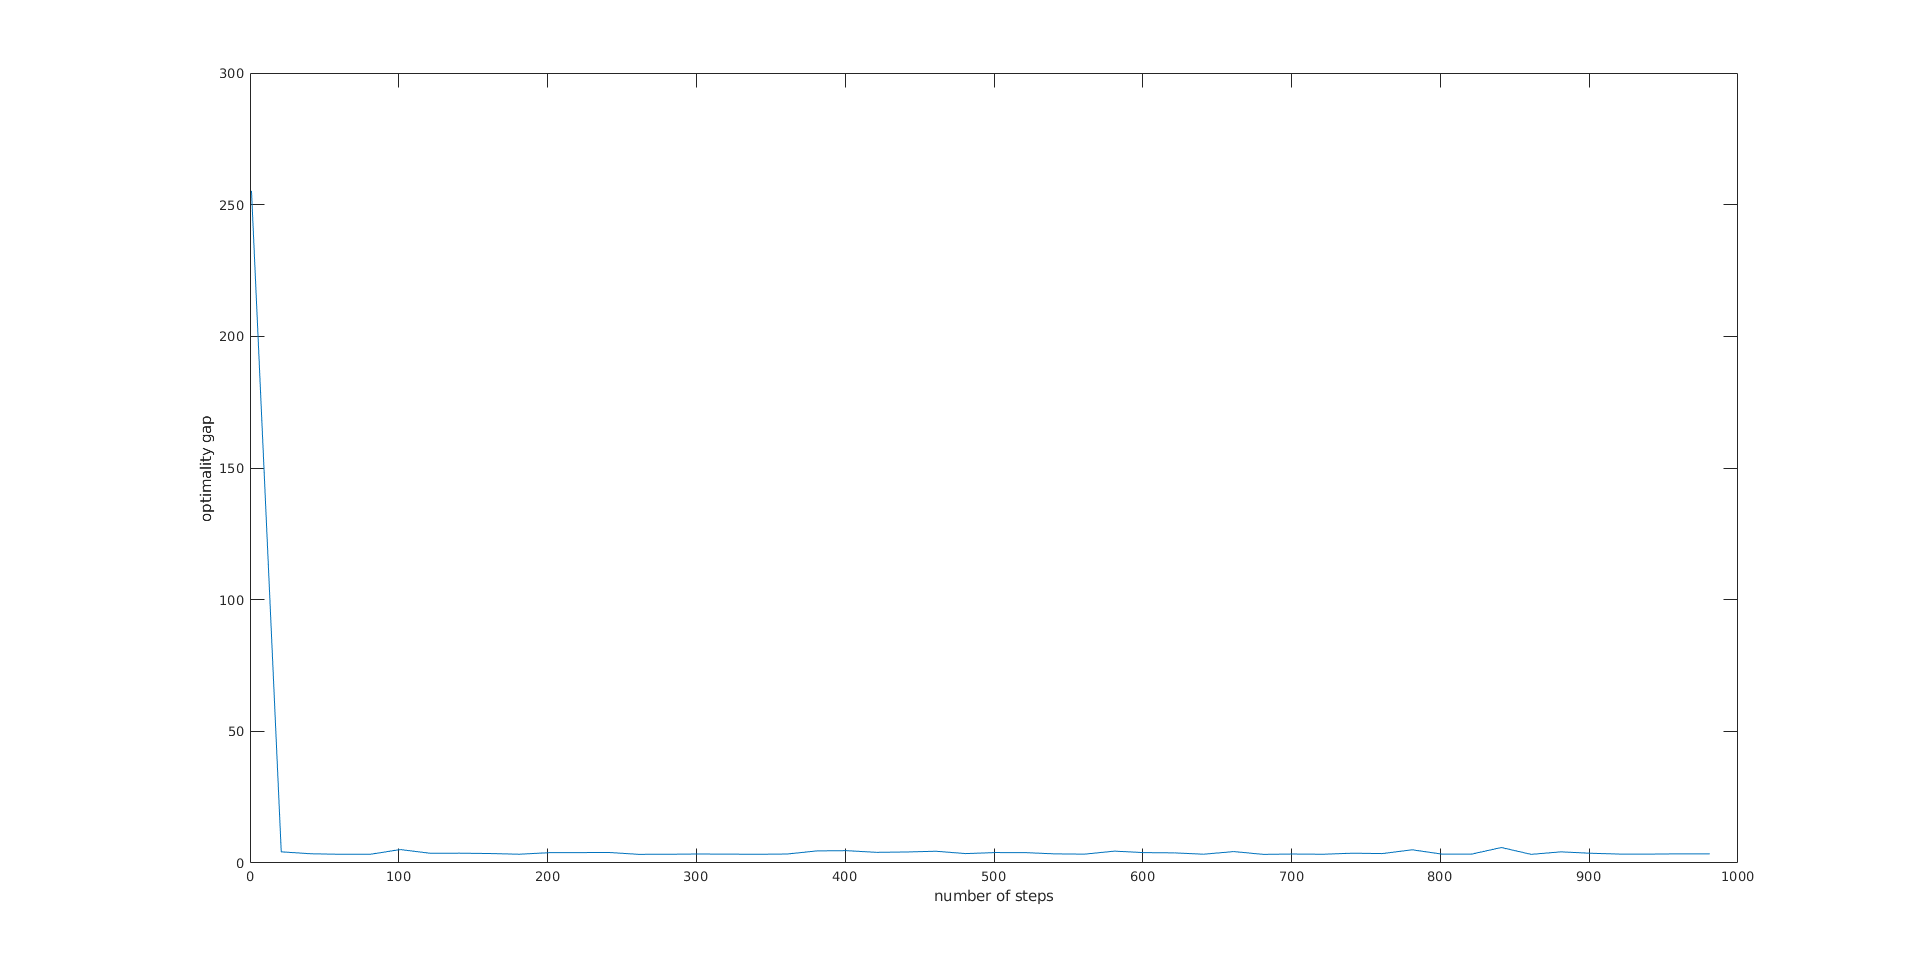
\includegraphics[scale=0.3]{figure/p1_1_1.png}
\caption{SGD method}
\label{p1_1}
\end{figure}

\subsection*{question2}
As the $\alpha$ increses, the optimality gap increses.

\begin{figure}[htbp]
\centering
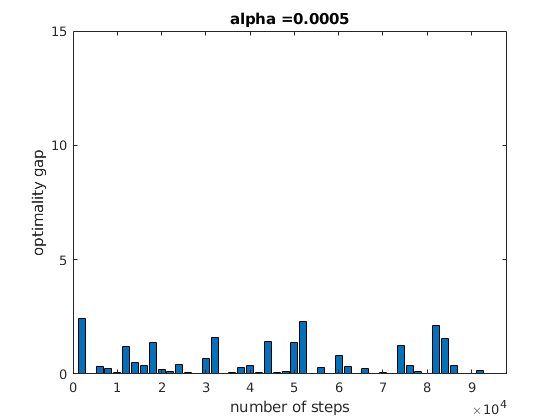
\includegraphics[scale=0.7]{figure/p1_2_1.png}
\caption{SGD method changing $\alpha$}
\label{p1_2_1}
\end{figure}

\begin{figure}[htbp]
\centering
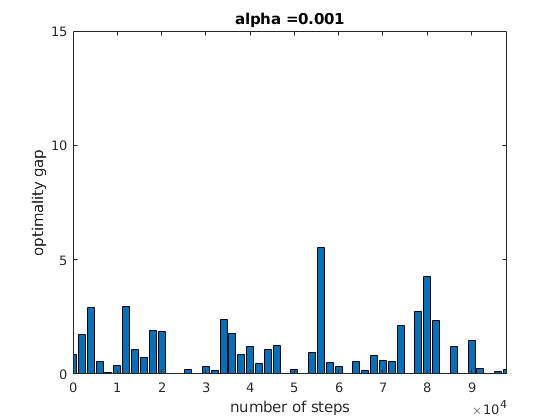
\includegraphics[scale=0.7]{figure/p1_2_2.png}
\caption{SGD method changing $\alpha$}
\label{p1_2_2}
\end{figure}

\begin{figure}[htbp]
\centering
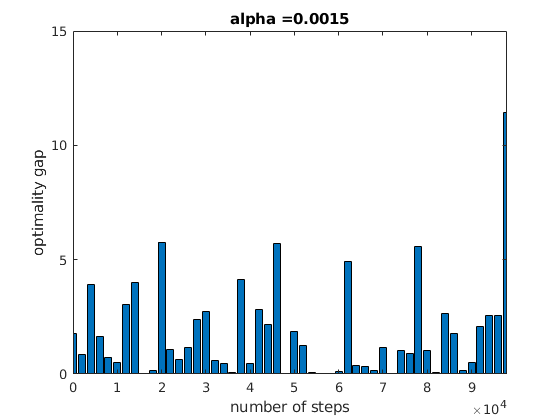
\includegraphics[scale=0.7]{figure/p1_2_3.png}
\caption{SGD method changing $\alpha$}
\label{p1_2_3}
\end{figure}

\begin{figure}[htbp]
\centering
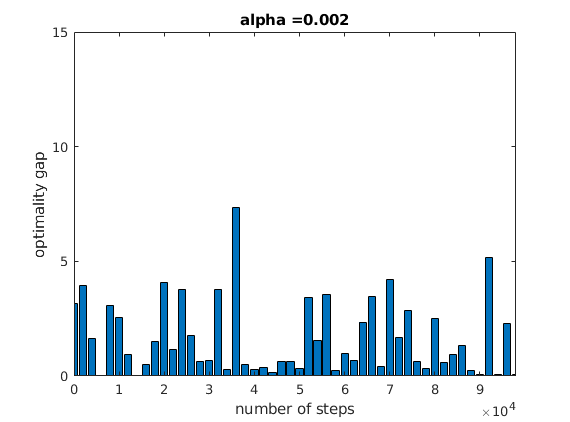
\includegraphics[scale=0.7]{figure/p1_2_4.png}
\caption{SGD method changing $\alpha$}
\label{p1_2_4}
\end{figure}

\begin{figure}[htbp]
\centering
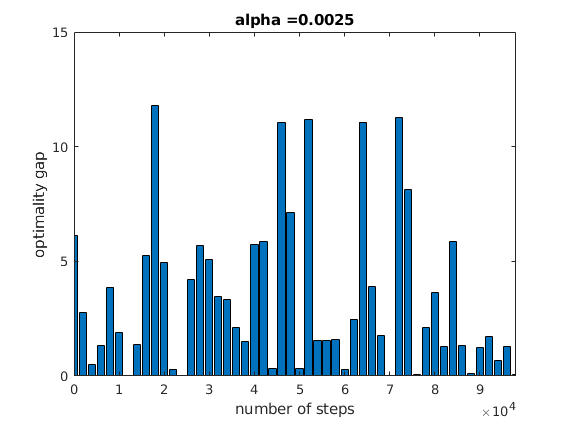
\includegraphics[scale=0.7]{figure/p1_2_5.png}
\caption{SGD method changing $\alpha$}
\label{p1_2_5}
\end{figure}

\begin{figure}[htbp]
\centering
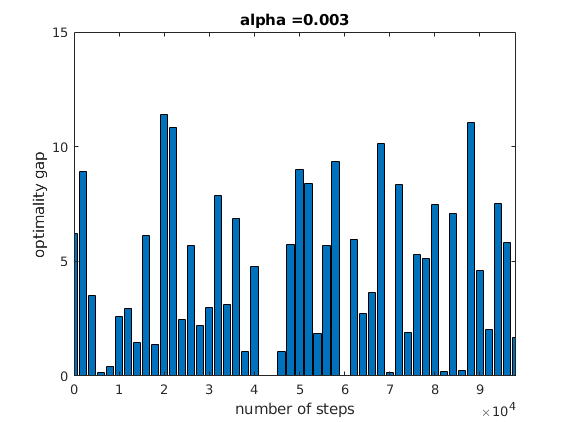
\includegraphics[scale=0.7]{figure/p1_2_6.png}
\caption{SGD method changing $\alpha$}
\label{p1_2_6}
\end{figure}

\begin{figure}[htbp]
\centering
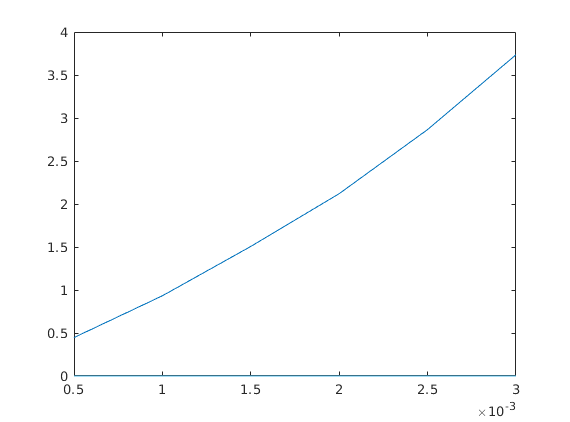
\includegraphics[scale=0.7]{figure/p1_2_7.png}
\caption{mean optimality gap v.s. $\alpha$ }
\label{p1_2_7}
\end{figure}

\newpage
\section*{Problem 2}
\subsection*{question1}
$log \rho(I) = 6.6613e-16$
\subsection*{question2}
With the sample sizes increses, the $log\rho(G)$ decreses.(almost linearly)
\begin{figure}[htbp]
\centering
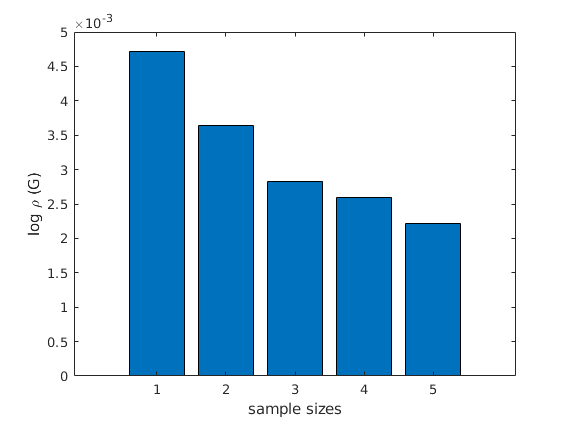
\includegraphics[scale=1]{figure/p2_2.png}
\caption{Gauss-Newton method}
\label{p2_2}
\end{figure}

\newpage
\section*{Problem 3}
The figure shows that Gauss-Newton method converges quicker than SGD method.
\begin{figure}[htbp]
\centering
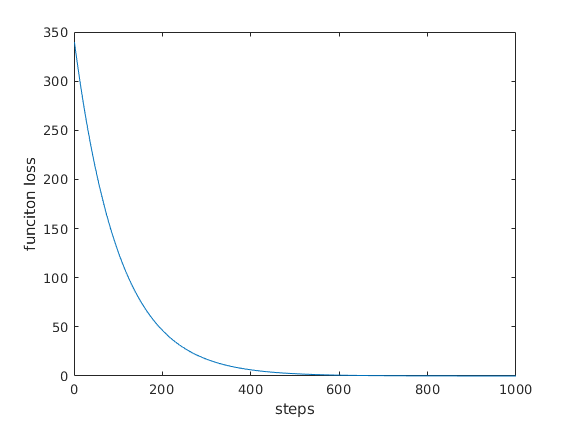
\includegraphics[scale=1]{figure/p3.png}
\caption{Gauss-Newton method}
\label{p3}
\end{figure}

\lstset{
	language=Octave,
	xleftmargin=3em,
	}
\begin{lstlisting}
load('cricket.dat');
A = cricket(:,1);
b = cricket(:,2);

A = [A, ones(length(b), 1)];

% ===== initial ===== %

max_step = 1000;
alpha = 0.005;
c = 0.0003;
threshold = 1e-4;

len = length(b);
phi = 0;
tmp = A*x-b;
for i = 1:len
	phi = phi + exp(tmp(i)^2);
end
phi = phi - 1;
% ===== iterate ===== %

x = [0; 0];
errors = zeros(1, max_step);

for i = 1:max_step
	r = b - A*x;

	df = -2 * c * exp(c*r.^2).*r.*A;
	f = exp(c*r.^2) - 1;

	p = -(df'*df) \ (df'*f);
	x = x + alpha * p;

	errors(i) = 0.5 * (f' * f);

	if norm(df, 2) < threshold
		break;
	end
end

x_step = 1:max_step;
plot(x_step, errors);
xlabel('steps');
ylabel('funciton loss');

\end{lstlisting}
\end{document}
